
%(BEGIN_QUESTION)
% Copyright 2010, Tony R. Kuphaldt, released under the Creative Commons Attribution License (v 1.0)
% This means you may do almost anything with this work of mine, so long as you give me proper credit

Calculate the appropriate LRV and URV pressures for this hydrostatic level measurement system, assuming the process liquid has a weight density of 55 pounds per cubic foot:

$$\includegraphics[width=15.5cm]{i03748x01.eps}$$

Express your answers in units of {\it PSI}.

\vskip 10pt

If this transmitter were replaced with another one having the exact same calibration but different fill fluid (S.G. = 0.951 instead of 1.07), how would its level-measurement accuracy be affected?

\underbar{file i03748}
%(END_QUESTION)





%(BEGIN_ANSWER)

LRV = +4.42 PSI \hskip 50pt URV = +1.74 PSI

\vskip 10pt

A fill fluid of lesser density would apply less hydrostatic pressure to the ``high'' side of the transmitter, making the transmitter ``think'' there was a greater level of process liquid in the vessel.  This would be a shift in the level measurement system's {\it zero} only.  This change would neither affect span nor linearity.

Specifically, the zero shift would be equivalent to 1.62 feet of level in the vessel!

%(END_ANSWER)





%(BEGIN_NOTES)


%INDEX% Measurement, level: hydrostatic pressure

%(END_NOTES)

